\subsection{Overview: High level components and their interaction}
The system is divided into three main layers: presentation layer, application layer and data layer. The presentation layer is the interface between the user and the system. It is responsible for the presentation of the data and the interaction with the user. The application layer is the core of the CKB Platform. It is responsible for the business logic and the communication between the presentation layer and the data layer. The data layer is responsible for the storage of the data. It is the interface between the application layer and the database.
\begin{figure}[H]
    \centering
    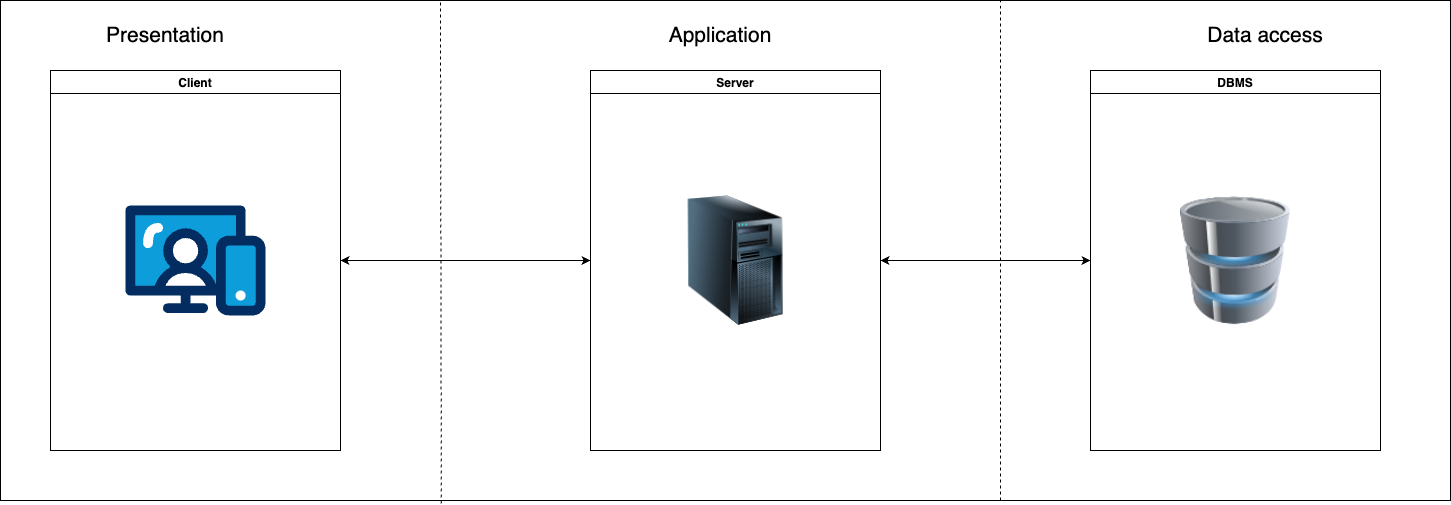
\includegraphics[width=\textwidth]{Images/three_tier.png}
    \caption{High level components and their interaction}
\end{figure}

The three-tier architecture was chosen for this type of system because of the several advantages it offers compared to other types of architectures. For that concerns scalability, it allows for easy scalability by separating the presentation, application, and data layers. Each layer can be scaled independently, allowing for better performance and resource utilization.
For what concers modulatiry, it promotes the separation of concers by dividing the system into distinct layers. This makes it easier to develop, test, and maintain each layer separately, improving overall code quality and reusability. The sepatarion of concerns also improves the maintainability of the system by providing clear boundaries between layers it makes easier to understand and modify specific parts of the system without affecting other layers.
The last advantage for which this architecture was chosen is flexibility. The three-tier provides flexibility in terms of technology choices. Each layer can be implemented using different technologies, allowing for the use of the most suitable tools and frameworks for each specific layer.

\begin{figure}[H]
    \centering
    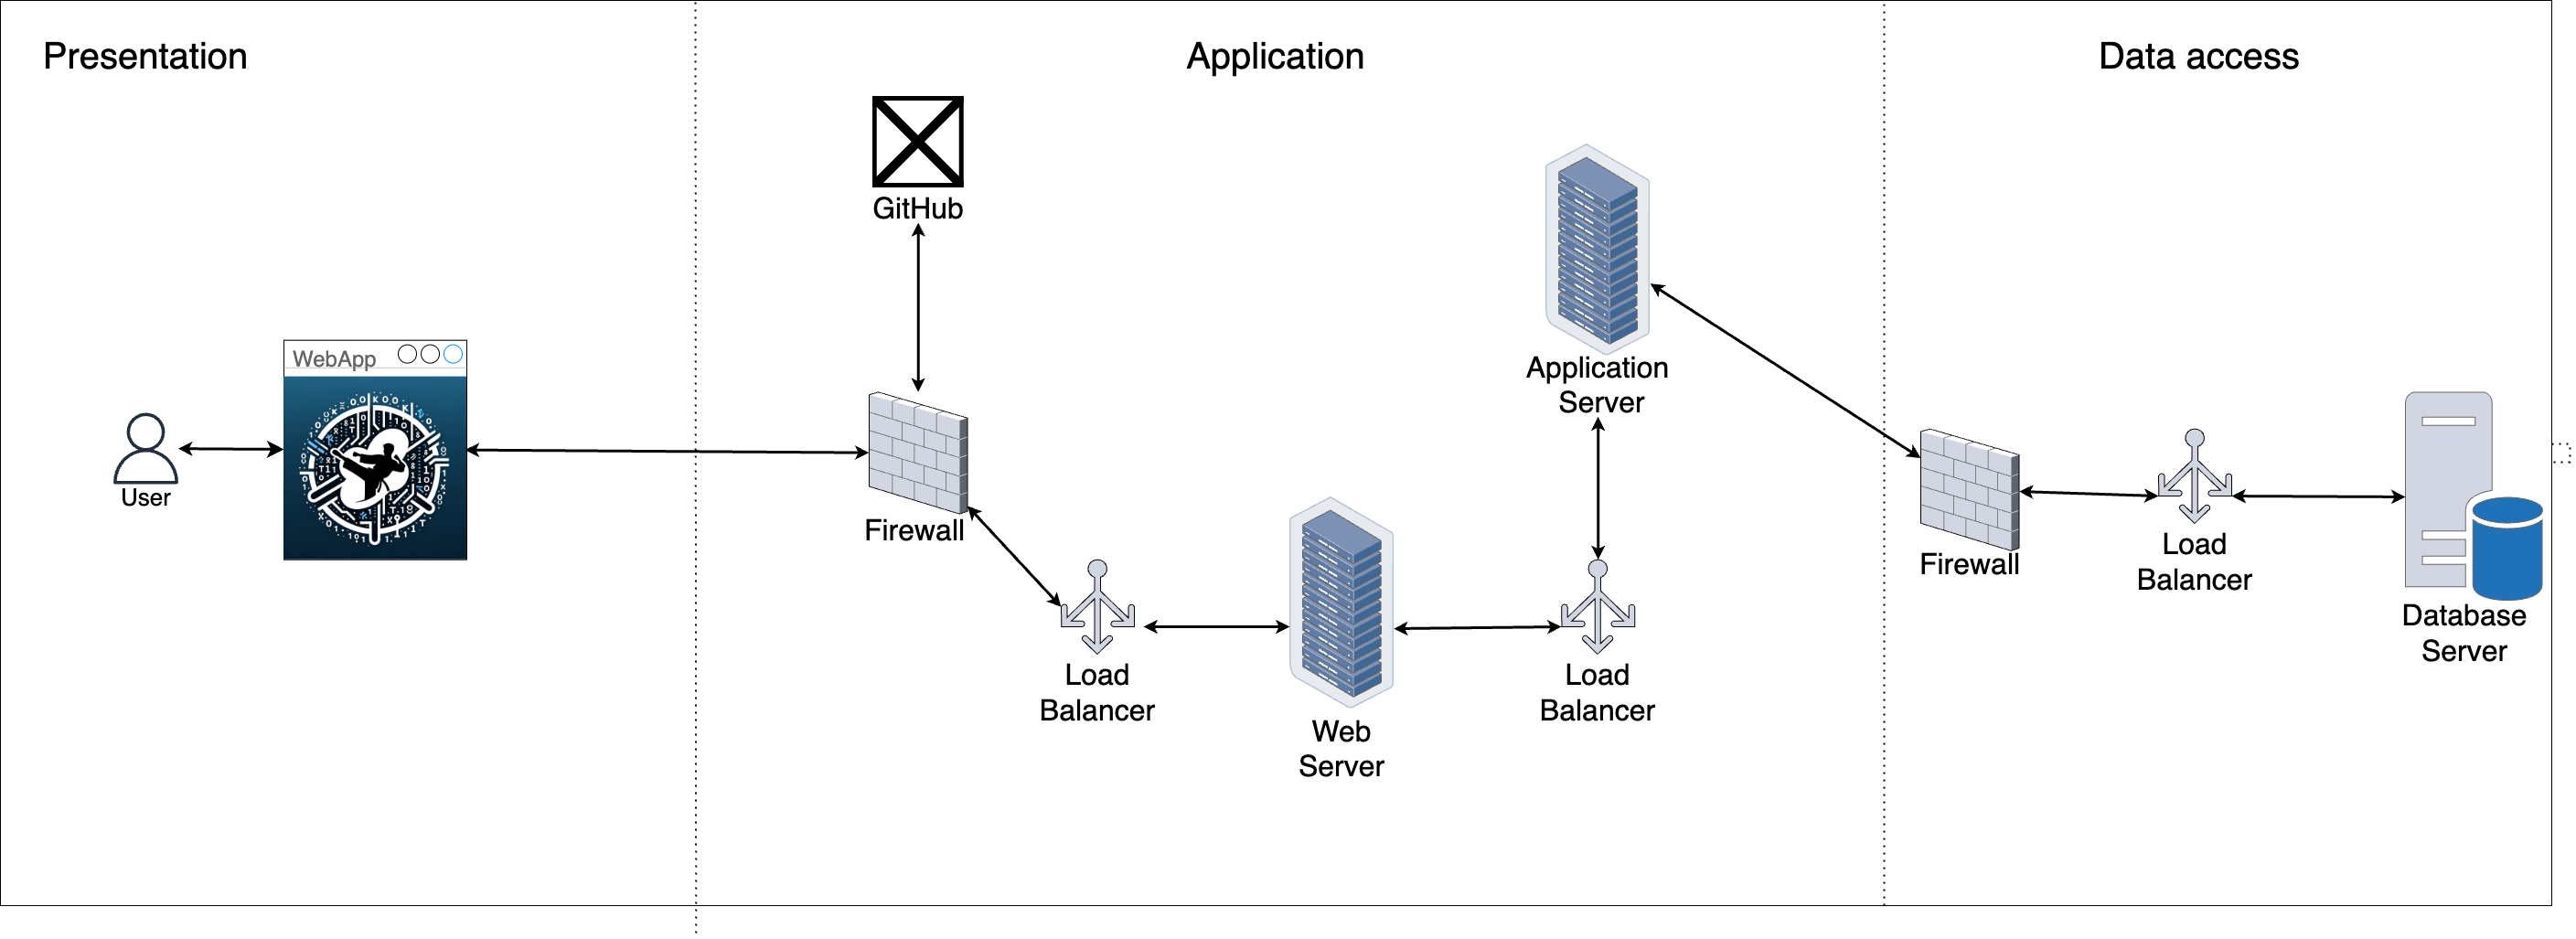
\includegraphics[width=\textwidth]{Images/high_level.png}
    \caption{High level system with interactions between the components}
    \label{fig:high_level_system}
\end{figure}

In the figure Figure\ \ref{fig:high_level_system} is shown the high level system with the interactions between the components. 
At the forefront is the Presentation layer, where a user engages with the web application through a web browser.
The web application depending on user interactions requests data from the web server. The interaction between the two is not direct since there is a firewall (for security reasons) and also a load balancer.

Moving inward, the Application layer serves as the system's operational core, where a network firewall establishes the first line of defense, safeguarding the internal processes. A load balancer stands right behind the firewall, directing incoming traffic to maintain system efficiency and reliability. This layer is further composed by an application server that executes the business logic, interfacing with databases or other external services as needed. Additionally, the presence of an upward arrow connecting the load balancer to GitHub to handle the evaluation trigger as well as the creation of the repositories. This is a very important feature of the system since it allows to automatically evaluate the students' submissions.

The final segment of the diagram is the Data Access layer, echoing the security and balance themes with its own firewall and load balancer, underscoring the system's commitment to secure data transactions. At the heart of this layer lies the database server, a robust storage solution that ensures data is efficiently stored, retrieved, and managed, completing the architecture's promise of a secure, scalable, and resilient web application environment.

\subsection{Component view}
In Figure\ \ref{fig:component_diagram} is shown the component diagram of the system. The system is divided into three main layers: presentation layer, application layer and data layer. The presentation layer is the interface between the user and the system and it is represented with the WebApp and Web Server Component. The application layer is the core of the CKB Platform and it is representend by the Application Server Subsystem. Finally the data layer is represented by the DBMS Component who is the only one that access the database.
\begin{figure}[H]
    \centering
    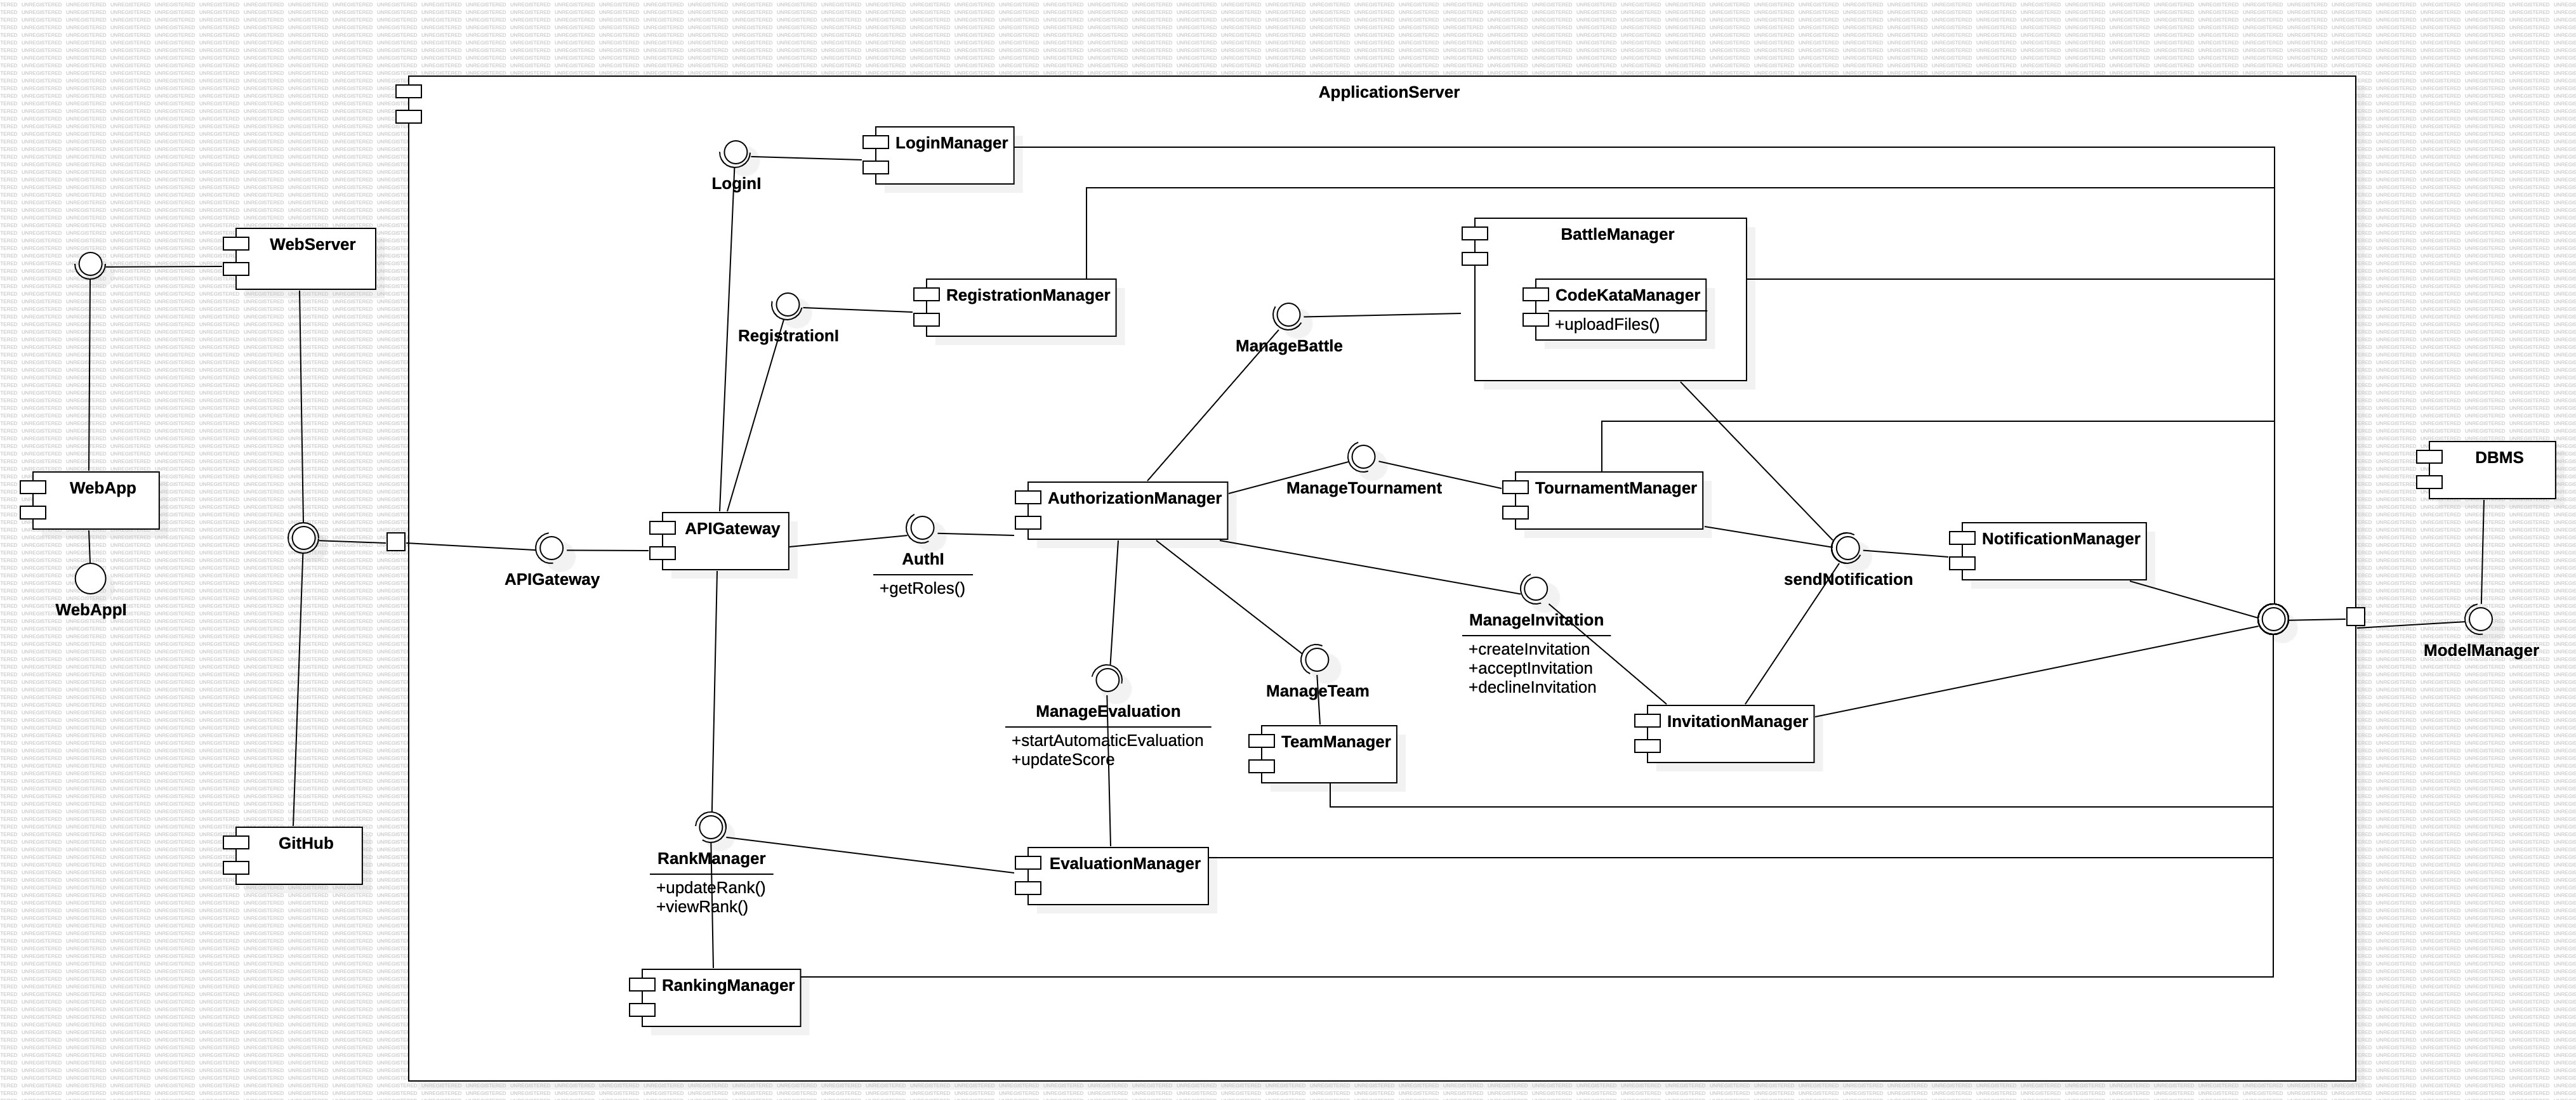
\includegraphics[angle=90,origin=c,width=0.6\textwidth]{Diagrams/ComponentDiagram.jpg}
    \caption{Component diagram}
    \label{fig:component_diagram}
\end{figure}
\clearpage
Regarding the presentation layer, it is represented by the following two components:
\begin{itemize}
    \item \textbf{WebApp}: it is the web application that the user interacts with. It is responsible for the presentation of the data and the interaction with the user. Since it communicates only with the Web Server, it can be executed by any device that has a web browser.
    \item \textbf{Web Server}: it is the component that handles the requests from the WebApp and forwards them to the Application Server. It is responsible to direct the requests to the APIGateway. It is also responsible to forward responses from the Application Server to the WebApp.
\end{itemize}
Regarding the application layer, it is represented by the components inside the Application Server Subsystem:
\begin{itemize}
    \item \textbf{APIGateway}: it is the component that handles the incoming requests to the Application Server. It is responsible to direct the requests to the correct component inside the Application Server Subsystem. It is also responsible to forward responses from the Application Server to the Web Server.
    \item \textbf{Login Manager}: it is the component that handles the login requests. It is responsible to check the credentials and to log the user in.
    \item \textbf{Registration Manager}: it is the component that handles the registration requests. It is responsible to create a new user.
    \item \textbf{Authorization Manager}: it is the component that handles the authorization requests. It is responsible to check if the user is authorized to perform the requested action. This is of paramount importance since only a user with Educator role can perform administrative actions, such as the creation of a new Tournament or Battle.
    \item \textbf{Evaluation Manager}: it is the component that handles the evaluation requests. It is responsible to evaluate the submissions of the students and to return the results. It performs the evaluation by running and testing the submissions provided by the students. It can be used also by the Educator to re-evaluate the submissions manually.
    \item \textbf{Ranking Manager}: it is the component that handles the rank of students in a Tournament.
    \item \textbf{Team Manager}: it is the component that handles the creation of teams and the assignment of students to teams. It is also responsible to guarantee that the restrictions on the number of students per team, set by the Educator, are respected.
    \item \textbf{Submission Manager}: it is the component that handles the submission of the students. The submission is created when the GitHub Action is triggered by the push of the student in the Team repository. It interacts with the Evaluation Manager to get the evaluation of the submission.
    \item \textbf{Invitation Manager}: it is the component that handles the invitation of both Students and Educator. In the case of the Students it is responsible to manage the invitation to join a Team. In the case of the Educator it is responsible to manage the invitation to join a Tournament.
    \item \textbf{Notification Manager}: it is the component that handles the notification requests. It is responsible to send notifications to the users. Such notifications are sent respecting the conditions previously specified in the RASD document.
    \item \textbf{Battle Manager}: it is the component that handles the creation and the management of Battles by the Educator. It is a complex component since it embodies also the CodeKata Manager. Since it contains the CodeKata Manager, it is responsible to handle the CodeKata files uploaded by the Educator. It interacts with the GitHub Component to create the repositories for the Battles. It also handles the different Battle phases, by guaranteeing the deadline restrictions set by the Educator.
    \item \textbf{Tournament Manager}: it is the component that handles the creation and the management of Tournaments by the Educator. It is responsible to handle the different Tournament phases, by guaranteeing the deadline restrictions set by the Educator.
\end{itemize}
Regarding the data layer, it is represented by the following component:
\begin{itemize}
    \item \textbf{DBMS}: it is the component that handles the access to the database. It is responsible to store and retrieve the data from the database. It is the only component that can access the database.
\end{itemize}
\subsection{Deployment view}
In this section is shown the deployment diagram of the system. The diagram is divided into three main tier: the presentation tier, the application tier and the data tier. 
\begin{figure}[H]
    \centering
    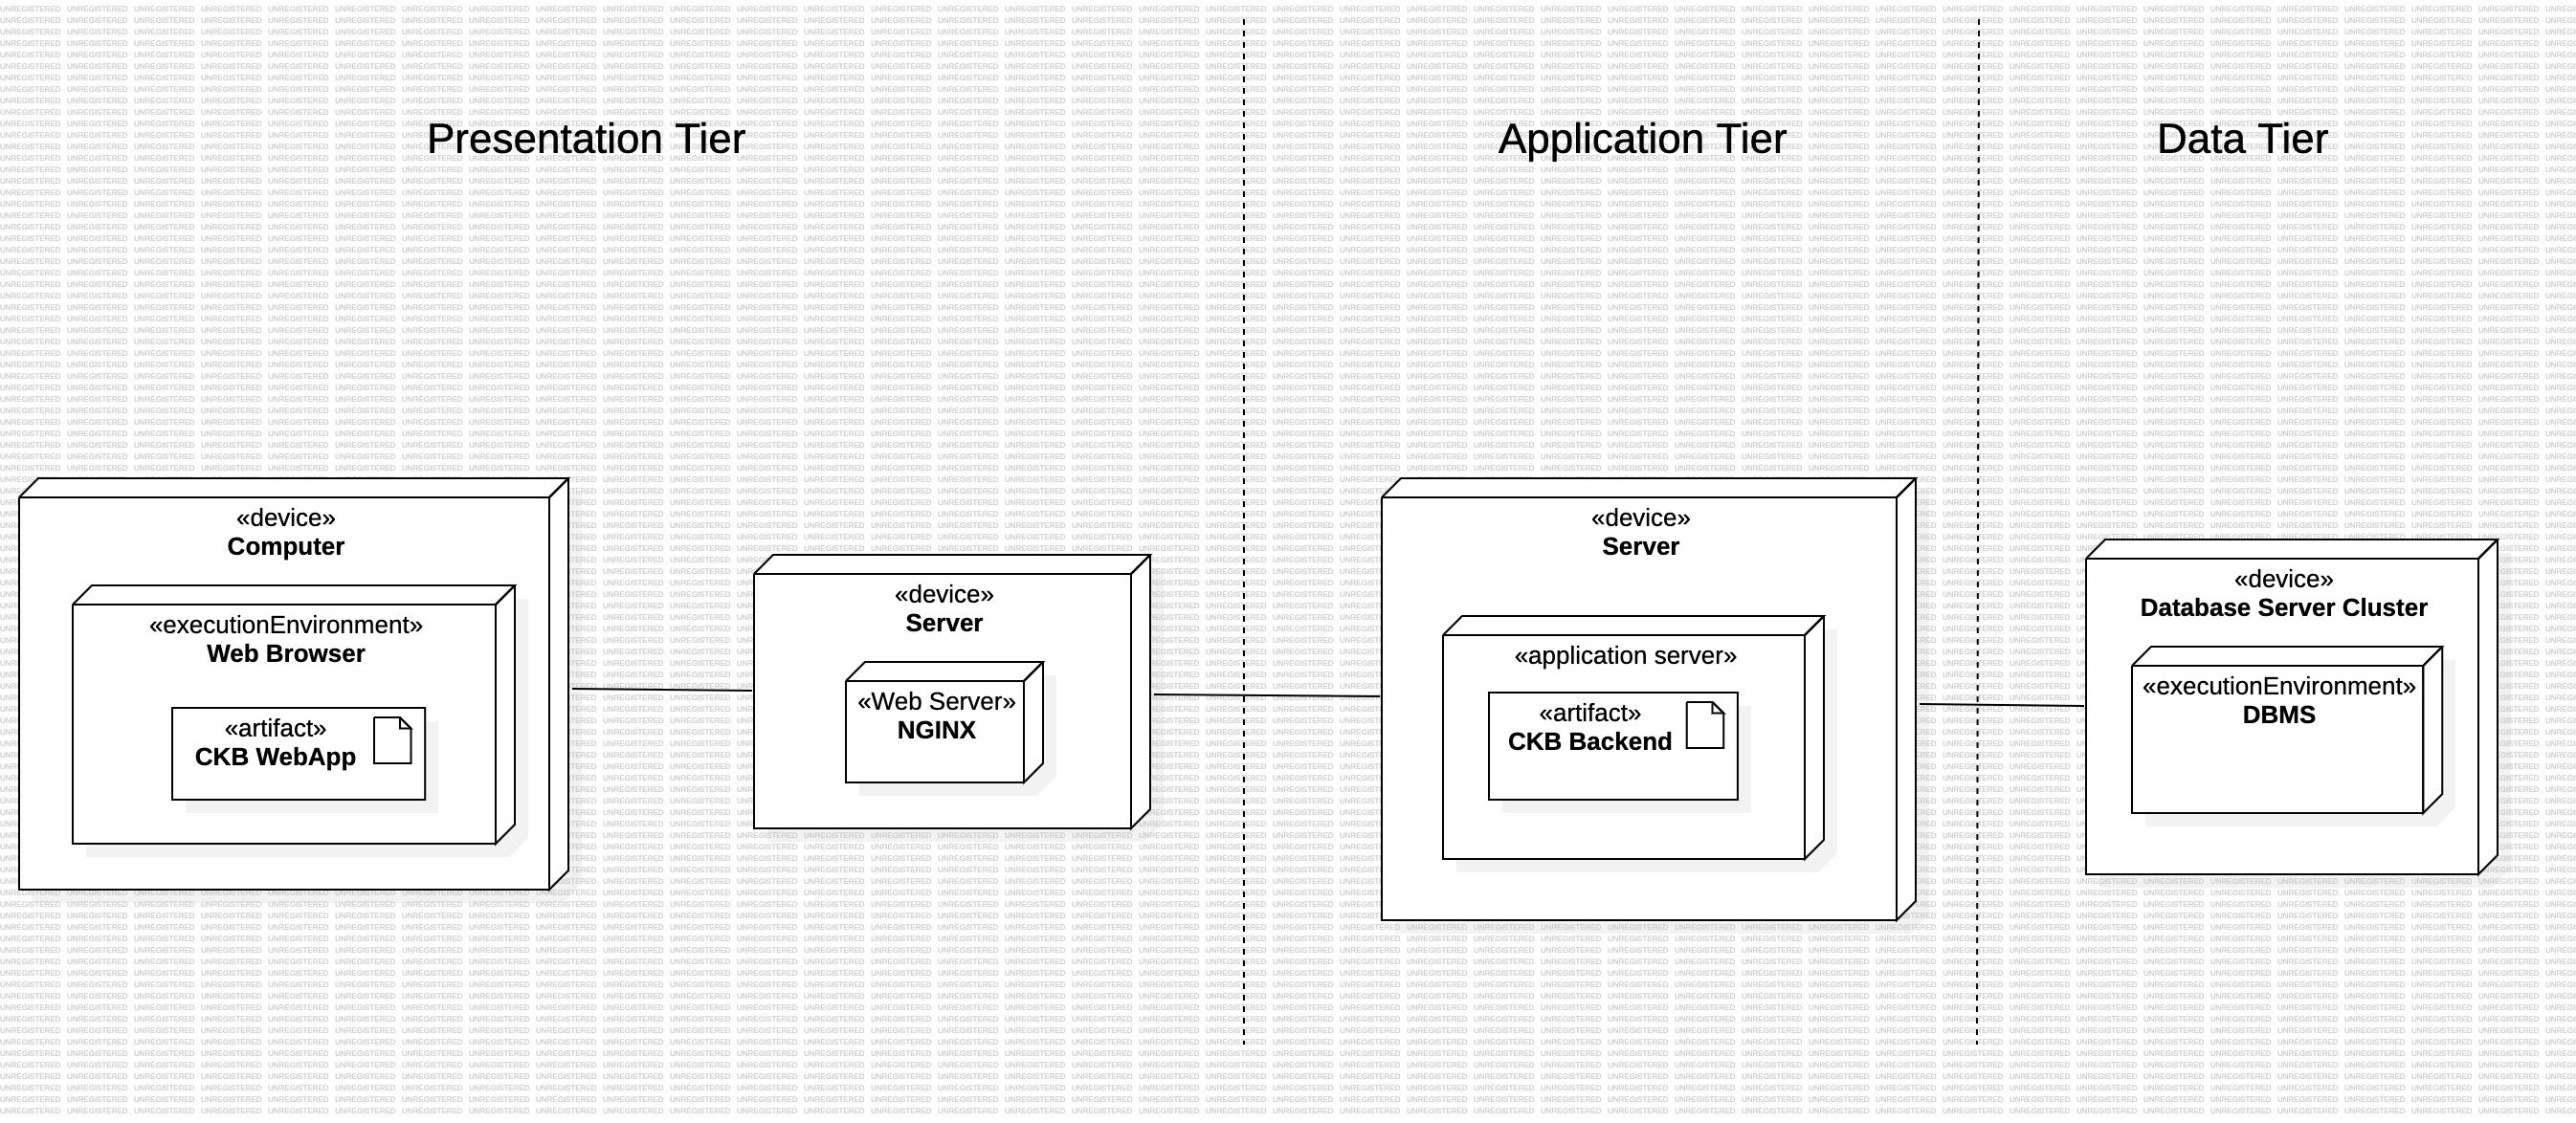
\includegraphics[width=\textwidth]{Diagrams/DeploymentDiagram.jpg}
    \caption{Deployment diagram}
    \label{fig:deployment_diagram}
\end{figure}
In figure Figure\ \ref{fig:deployment_diagram} is shown the deployment diagram of the system.
Regarding the presentation tier, it is represented by the following components:
\begin{itemize}
    \item \textbf{Computer}: it is a normal computer used by the user. It is the device that the user uses to interact with the CKB WebApp. It has no particular requirements since it only needs a web browser to access the WebApp.
    \item \textbf{Web Browser}: it is the software that the user uses to interact with the CKB WebApp. The CKB platform has to support the most common web browsers, such as Google Chrome, Mozilla Firefox, Microsoft Edge and Apple Safari.
    \item \textbf{CKB WebApp}: it is the web application that the user interacts with and it is used within the web browser. It is responsible for the presentation of the data and the interaction with the user.
    \item \textbf{Web Server}: it is a server that hosts a NGINX web server instance. The choice of NGINX is due to its high performance, low memory usage and high availability.
\end{itemize}
Regarding the application tier, it is represented by the following components:
\begin{itemize}
    \item \textbf{Application Server}: it is a server that hosts a CKB Backend application instance. It receives the requests from the Web Server and forwards it to the CKB Backend. At the same time it provides responses to the Web Server. It is also responsible to communicate with the DBMS to retrieve and store data.
    \item \textbf{CKB Backend}: it is the backend application of the CKB Platform. It handle the entire business logic of the application. It is responsible to process the forwarded requests and to provide responses to the Application Server.
\end{itemize}
Regarding the data tier, it is represented by the following components:
\begin{itemize}
    \item \textbf{Database Server Cluster}: it is a cluster of servers that hosts a DBMS instance. The choice of a cluster is due to the fact that it provides high availability and scalability. It is also responsible to guarantee the security of the data. It process the database specific requests sent by the Application Server.
    \item \textbf{DBMS}: it is the software that manages the database. It is responsible to store and retrieve the data from the database. It is the only component that can access the database.
\end{itemize}
\subsection{Component interfaces}

\textbf{Interface} LoginManager:
\begin{itemize}
    \item \texttt{Session login(String username, String password);}
    \item \texttt{void logout(Session session);}
\end{itemize}

\textbf{Interface} RegistrationManager:
\begin{itemize}
    \item \texttt{boolean register(UserDetails userDetails);}
\end{itemize}

\textbf{Interface} AuthorizationManager:
\begin{itemize}
    \item \texttt{List<Role> getRoles(User user);}
    \\ Get the roles of a user. The roles are used to determine if a user is authorized to perform a specific action.
\end{itemize}

\textbf{Interface} BattleManager:
\begin{itemize}
    \item \texttt{Battle createBattle(BattleDetails details);}
    \\ Create a new Battle. The BattleDetails contains all the information needed to create a new Battle.
    \item \texttt{boolean uploadFiles(Battle battle, CodeKata files);}
    \\ Upload the files of the CodeKata. The files must contain the tests and the automation scripts of the CodeKata.
    \item \texttt{boolean updateBattle(Battle battle, BattleDetails details);}
    Updates the details of a Battle, such as the different stages and the deadlines.
    \item \texttt{List<Team> getTeams(Battle battle);}
\end{itemize}

\textbf{Interface} TournamentManager:
\begin{itemize}
    \item \texttt{Tournament createTournament(TournamentDetails details);}
    \\ Create a new Tournament. The TournamentDetails contains all the information needed to create a new Tournament.
    \item \texttt{boolean updateTournament(Tournament tournament, TournamentDetails details);}
    \\ Updates the details of a Tournament, such as the different stages and the deadlines.
\end{itemize}

\textbf{Interface} InvitationManager:
\begin{itemize}
    \item \texttt{boolean sendInvitation(User user, Invitation invitation);}
    \\ Send an invitation to a user. The invitation can be to join a Tournament, if the user is an Educator, or to join a Team, if the user is a Student.
    \item \texttt{boolean acceptInvitation(Invitation invitation);}
    \\ Accept an invitation sent by another user.
    \item \texttt{boolean declineInvitation(Invitation invitation);}
    \\ Decline an invitation sent by another user.
\end{itemize}

\textbf{Interface} RankingManager:
\begin{itemize}
    \item \texttt{void updateRank(Student student, Tournament tournament, int newRank);}
    \\ Update the rank of a Student in a Tournament. This method can only be used by users with Educator Role.
    \item \texttt{int viewRank(Student student, Tournament tournament);}
    \\ View the rank of a Student in a Tournament.
\end{itemize}

\textbf{Interface} SubmissionManager:
\begin{itemize}
    \item \texttt{SubmissionResult submit(Item item);}
    \\ Submit a solution to a Battle. The Item contains the code of the solution. The SubmissionResult contains the evaluation of the submission.
    \item \texttt{Item getSubmission(int submissionId);}
    \\ Get the code of a submission given its id.
    \item \texttt{SubmissionResult getSubmissionResult(int submissionId);}
    \\ Get the evaluation of a submission given its id.
\end{itemize}

\textbf{Interface} NotificationManager:
\begin{itemize}
    \item \texttt{void notify(User user, Notification notification);}
    \\ Send a notification to a user.
\end{itemize}

\textbf{Interface} ModelManager:
\begin{itemize}
    \item \texttt{boolean saveModel(DataModel model);}
    \\ Save a DataModel in the database.
    \item \texttt{DataModel getModel(DataModel model, List<Filter> filters);}
    \\ Get a DataModel from the database given its id.
    \item \texttt{boolean updateModel(DataModel model);}
    \\ Update a DataModel in the database.
    \item \texttt{boolean deleteModel(DataModel model);}
    \\ Delete a DataModel from the database.
\end{itemize}

\textbf{Interface} TeamManager:
\begin{itemize}
    \item \texttt{Team createTeam(TeamDetails details);}
    \\ Create a new Team. The TeamDetails contains all the information needed to create a new Team.
    \item \texttt{boolean updateTeam(Team team, TeamDetails details);}
    \\ Updates the details of a Team, such as the name and the members.
    \item \texttt{boolean addMember(Team team, Student student);}
    \\ Add a Student to a Team.
\end{itemize}
\subsection{Runtime view}
In this section are shown the sequence diagrams of the main functionalities of the system previously described in the RASD document. Starting from the \textit{Component View} section of this document, it is possible to identify the components interactions that are shown in the following sequence diagrams.
\subsubsection*{Login}
\begin{figure}[H]
    \centering
    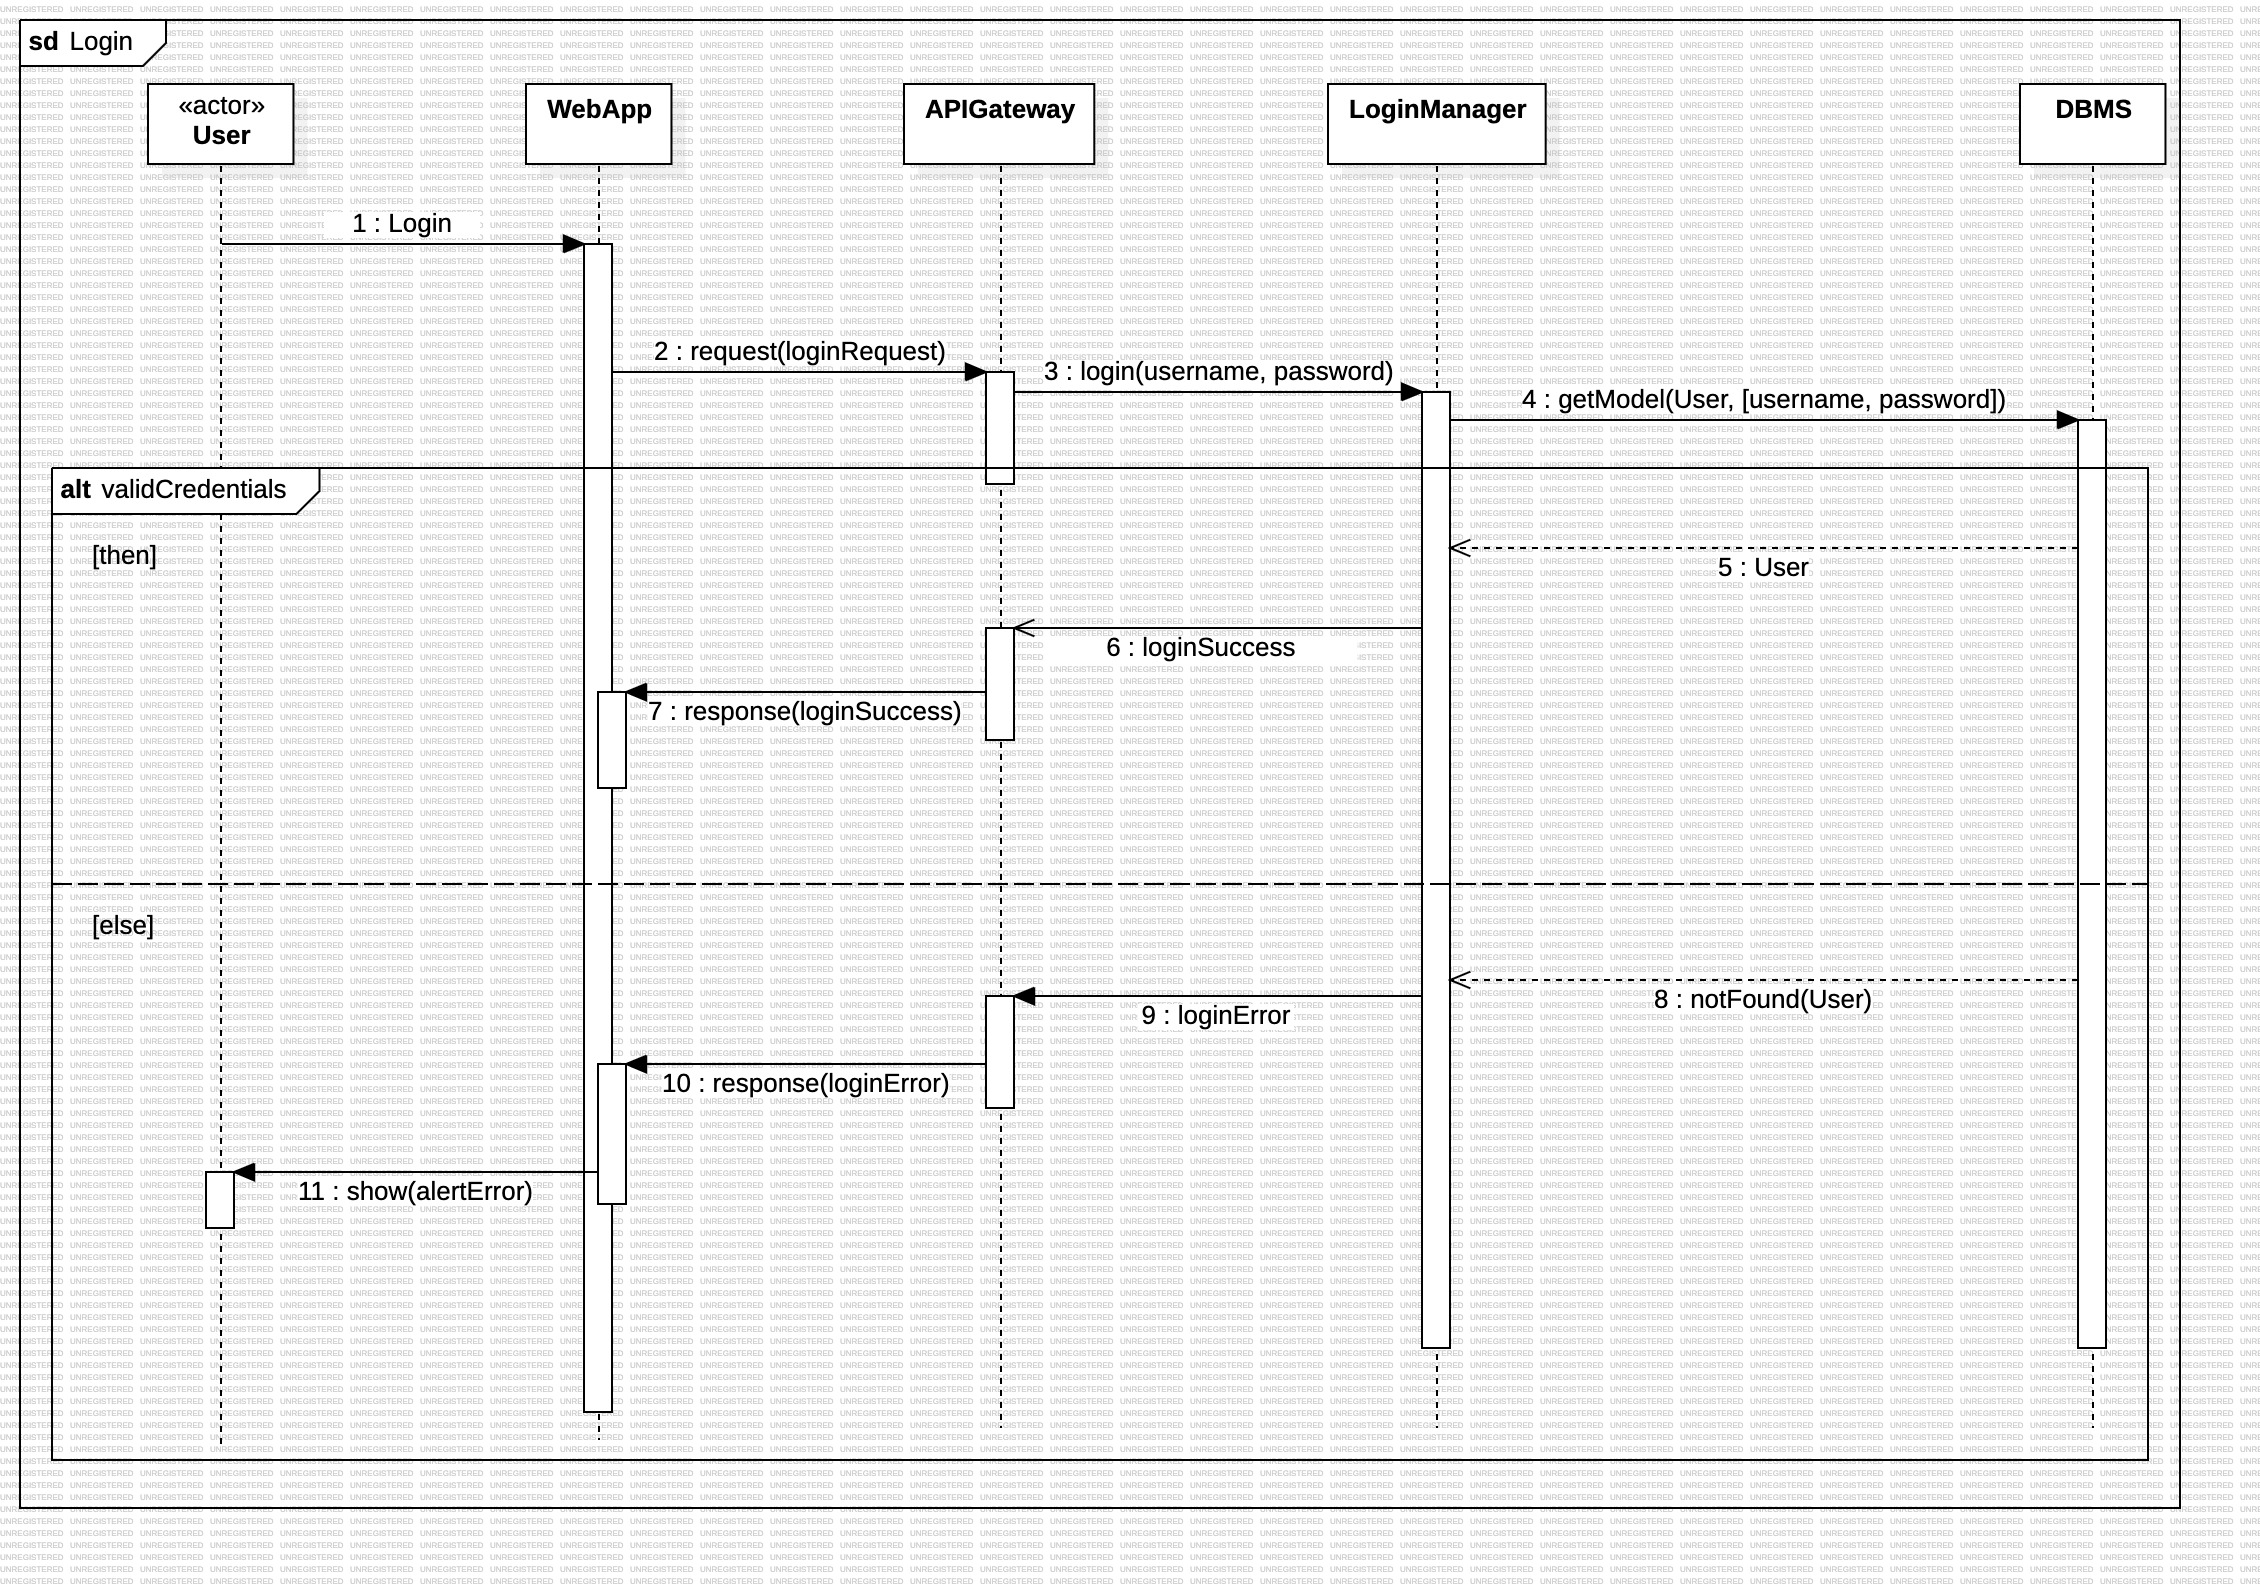
\includegraphics[width=\textwidth]{Diagrams/LoginSD.jpg}
    \caption{Runtime view}
    \label{fig:runtime_view}
\end{figure}
\subsection{Selected architectural styles and patterns}
\subsection{Other design decisions}
